\chapter{Introducción} \label{chap:Introduccion}
\chapterimage{figuras/ImagenesPortada/PortadaIntro.jpg}
\hrule
\vspace{3mm}

En este capítulo se perfila la estructura, organización y contenidos principales del documento así como la motivación y objetivos del proyecto.


\section{Motivación del proyecto}



\section{Objetivos}

El objetivo que este Trabajo de Fin de Grado persigue es el del diseño, construcción y control de brazo robótico previo estudio de las opciones comerciales disponibles y su posible adaptación. Este proyecto está enmarcado bajo el proyecto Robohealth, proyecto financiado por el Ministerio de Economía y Competitividad con el objetivo del diseño de sistemas robóticos y domóticos para entornos hospitalarios que mejoren el sistema de salud actual. (\completar http://robohealth.es/)
\\

El  prototipo debe estar diseñado para una completa adaptación a un entorno hospitalario en el que deberá estar en contacto constante con usuarios a los que deberá respetar.
\\

El objetivo del brazo robótico es el de ubicar ante un paciente una \ingles{tablet}. Ésta llevará montado un dispositivo de seguimiento de vista de forma que, a través del movimiento de las pupilas, el paciente podrá interactuar con el resto de dispositivos de la habitación así como el personal médico. Es necesario motorizar el dispositivo para mantener el dispositivo de seguimiento siempre a una distancia y ángulo, respecto a la cara del paciente, mínima para facilitar el funcionamiento del mismo. Está pensado principalmente para pacientes con movilidad reducida o sin movilidad (temporal o permanente), aunque también podría agilizar la interfaz humano-habitación para el resto de pacientes.
\\

Así pues, algunos aspectos claves del prototipo deben ser:
\begin{itemize}
    \item El Objetivo del prototipo será el de permitir una interacción más cómoda y automatizada entre los pacientes cuya capacidad de interacción se ha visto reducida por la causa que sea.
    \item Se debe tener en cuenta es que el prototipo estará en constante contacto con gran variedad de usuarios: pacientes, médicos, familiares, etc. El diseño debe proteger en todo momento la seguridad de dichos usuarios
    \item Concretamente el diseño está pensado para interactuar con pacientes que se encuentran recostados en una camilla en el hospital.
\end{itemize}

\subsection{Objetivos derivados}

La realización de dicho prototipo implica el cumplimiento de otros objetivos secundarios o derivados del principal. Se pueden listar algunos como:
\begin{itemize}
    \item Prueba de diferentes tipos de estructuras y materiales como base física del brazo robótico.
    \item Adquisición de conocimientos sobre modelado 3D digital así como diferentes métodos de fabricación como son la impresión 3D, el corte láser, fresado CNC así como el uso de otras herramientas de mecanizado más tradicionales.
    \item Diseño e implementación de un sistema de control en cascada, que permita un control en posición y en velocidad del brazo robótico.
\end{itemize}


\section{Estructura del documento}

El documento está organizado de tal forma que irá introduciendo al lector progresivamente en los diferentes aspectos del diseño y montaje del prototipo mencionado, desde aspectos más generales hasta los más técnicos.
\\

Los capítulos están a su vez organizados en el orden que se seguiría de cara a montar el prototipo empezando por una base física, añadiendo a posteriori los componentes electromecánicos para finalizar con los aspectos de control. Concretamente los capítulos contienen la siguiente información:

\begin{itemize}
    \item Como continuación de los requerimientos generales se encuentra descritos en la introducción, en el capítulo \ref{chap:estadoarte}, un estudio de diferentes modelos y diseños comerciales que podrían adaptarse para cumplir los objetivos presentados.
    \item El estudio del estado del arte ayuda a definir las ideas más importantes que regirán el diseño del prototipo. Éstas consideraciones se presentan en el capítulo \ref{chap:Punto_partida}.
    \item El capítulo \ref{chap:Mecanica} entra de lleno en los aspectos mecánicos del brazo robótico, pasando por una valoración de distintas posibilidades para llegar al diseño definitivo.
    \item Continuando con la descripción de soporte físico, el capítulo \ref{chap:Cinematica} supone un cambio de perspectiva que guiará al lector desde la parte mecánica y física expuesta anteriormente a la descripción matemática y cinemático del modelo.
    \item Una vez descrito el soporte físico del brazo robótico se detalla el hardware escogido para su puesta en marcha. En el capítulo \ref{chap:Electronica} presentan los componentes electromecánicos que se han integrado en prototipo; sus características principales así como su ubicación en el montaje.
    \item El análisis de la estructura software diseñado queda cubierto en el capítulo \ref{chap:SW}. Este apartado anticipa además algunas ideas sobre el sistema de control diseñado.
    \item Continuando con las pinceladas aportadas en el apartado anterior, el capítulo \ref{chap:Control} expone de forma detallada los distintos aspectos de diseño y desarrollo del control del brazo.
    \item Una vez alcanzado este punto, habiendo cubierto los aspectos del diseño del brazo, el capítulo \ref{chap:Resultados} recoge los resultados de funcionamiento de prototipo para ser analizados.
    \item No se dejan de lado aspectos de gestión, costes y viabilidad del prototipo que se detallan en el capítulo \ref{chap:Gestion}.
    \item Finalmente, el capítulo \ref{chap:Conclusiones} expone las conclusiones finales del trabajo así como posibles desarrollos futuros.
\end{itemize}

Como complemento a la información que exponen los apartados de esta memoria se añaden al final diferentes anexos:

\begin{itemize}
    \item Se adjunta un listado de todas las piezas diseñadas con información relevante sobre su uso y fabricación en el anexo \ref{app:listadoPiezas}.
    \item Vistas las piezas que conforman el prototipo es importante localizarlas para entender su uso y diseño. El anexo \ref{app:montajePiezas} detalla unas pautas y orden para el ensamblado del prototipo. Además permite localizar en su contexto las piezas listadas en el anexo \ref{app:listadoPiezas}.
    \item Volviendo sobre los aspectos del software, en el Anexo \ref{app:codificacionSW} se concretan las reglas de codificación, mencionadas en el capítulo \ref{chap:SW}, más relevantes que se han aplicado en el desarrollo del código.
    \item De igual forma se amplia la información sobre el software desarrollado en el anexo \ref{app:documentacion_software}. En él se encuentra la documentación del software generada a través de la herramienta \glosario{doxygen}.
    \item El desarrollo del proyecto conlleva la utilización de diferentes herramientas software cuya instalación y puesta apunto se detalla en el anexo \ref{app:instalacion_software}.
\end{itemize}

\section{Software utilizado}

Aunque en el anexo \ref{app:instalacion_software} se detalla la instalación del software en más detalle no está de más conocer las herramientas a utilizar de antemano, ya que éstas marcan unas pautas en la ideología de diseño y una estructura a la hora de ordenar y desarrollar el proyecto.

\begin{itemize}
    \item Autodesk Inventor 2016: Es un software de modelado paramétrico 3D de la compañía Autodesk Inc.
    \item Atom: Se trata de un editor de texto \ingles{open source}. Permite la instalación de diferentes extensiones para ampliar sus utilidades, entre otras será necesario instalar \glosario{PlatformIO}, que convierte el editor en un \glosario{IDE} completo para el desarrollo de software para diferentes placas como Arduino, que será la base de este proyecto.
    \item Matlab: herramienta de cálculo utilizada para analizar la información recogida del ámbito de control así como para las comprobaciones pertinentes sobre la cinemática.
    \item Lizard: Software que permite el análisis de la complejidad de código. Se compone de una serie de scripts en python que, al ser ejecutados devuelven un fichero con métricas de complejidad referentes a los ficheros de código sobre los que se invoca: complejidad ciclomática, número de funciones en cada fichero, líneas de código en cada función y fichero, entre otras..
    \item Cloc: Es una herramienta sencilla que cuenta, de forma más precisa, el número de líneas de código, comentarios y líneas en blanco de los ficheros de código.
    \item cpplint: Análisis del cumplimiento de las reglas de codificación en el software. Es una herramienta desarrollada en python por Google LLC para asegurar que los proyectos cumplen con sus reglas de codificación, que se han seguido de forma parcial en este proyecto. Se pueden ver los aspectos más relevantes de las reglas de codificación en el Anexo \ref{app:codificacionSW}.
    \item doxygen: Permite la generación de documentación para código de diferentes lenguajes, c++ en este caso, de forma automática. La herramienta obtiene comentarios del código, escritos con una sintaxis determinada, para documentar los diferentes métodos, objetos y estructura del software.
\end{itemize}

Además es interesante repasar los términos que se incluyen en el Glosario y que aparecerán referenciados a lo largo del documento. \completar

\section{Iconografía del proyecto}

Se han diseñado y utilizado diferentes iconos que pueden servir para orientar el propósito o temática de las diferentes figuras incluidas en el documento así como el capítulo al que pertenecen, manteniendo un color uniforme a lo largo de cada capítulo. Además de tener en la figura \ref{fig:introduccion:iconos} una recopilación de los mismos, a continuación se expone una lista con su significado y capítulo al que se asocia.


\begin{multicols}{2} 
	\begin{flushleft} 
		\subsection*{Capítulo 1: Introducción}
		\inconExplanation{intro_yellow}{Introducción, apertura del proyecto}
	\end{flushleft}	
		
	\begin{flushright} 
		\subsection*{Capítulo 2: Estado del arte}
		\inconExplanation{arte_blue}{Aspectos relacionados con el estado del arte}
	\end{flushright}
\end{multicols} 

\subsection*{Capítulo 3: Punto de inicio del diseño}
\begin{multicols}{2} 
	\begin{flushleft} 
		\inconExplanation{lupa_yellow}{Detalles sobre el robot}
	\end{flushleft}	
	
	\begin{flushright} 
		\inconExplanation{idea_yellow}{Ideas de interés}
	\end{flushright}
\end{multicols} 

\subsection*{Capítulo 4: Mecánica}
\begin{multicols}{2} 
	\begin{flushleft} 
		\inconExplanation{brazo_red}{Aspectos generales de la estructura del brazo robótico}
	\end{flushleft}
	
	\begin{flushright} 
		\inconExplanation{mecanismo_red}{Transmisión mecánica de movimiento}
	\end{flushright}	
\end{multicols} 

\subsection*{Capítulo 5: Electromecánica}
\begin{multicols}{2} 
	\begin{flushleft} 
		\inconExplanation{motor_green}{Actuadores para el brazo robótico}
	\end{flushleft}
	
	\begin{flushright} 
		\inconExplanation{bateria_green}{Alimentación y etapas de potencia}
	\end{flushright}
\end{multicols} 
\begin{multicols}{2}
	\begin{flushleft} 
		\inconExplanation{velocidad_green}{Sensores para el brazo robótico}	
	\end{flushleft}
\end{multicols} 

\subsection*{Capítulo 6: Estudio matemático}
\begin{multicols}{2} 
	\begin{flushleft} 
		\inconExplanation{math_red}{Ecuaciones y relaciones matemáticas}
	\end{flushleft}
	
	\begin{flushright} 
		\inconExplanation{abaco_red}{Resultados calculados}
	\end{flushright}
\end{multicols} 

\begin{multicols}{2} 
	\begin{flushleft} 
		\subsection*{Capítulo 7: Aspectos de Control}
		\inconExplanation{control_yellow}{Gráficas y aspectos del control}
	\end{flushleft}
\end{multicols} 

\subsection*{Capítulo 8: Software}
\begin{multicols}{2} 
	\begin{flushleft} 
		\inconExplanation{llaves_blue}{Diseño y desarrollo del software}
	\end{flushleft}
	
	\begin{flushright} 
		\inconExplanation{debug_blue}{Test, verificación y debug del software desarrollado}
	\end{flushright}	
\end{multicols} 

\begin{multicols}{2} 
	\begin{flushleft} 
		\subsection*{Capítulo 9: Resultados y discusión}
		\inconExplanationOne{megafono_red}
	\end{flushleft}
	\begin{flushright} 
		\subsection*{Capítulo 10: Gestión del proyecto}
		\inconExplanation{agenda_green}{Aspectos relacionados con el estado del arte}
	\end{flushright}
\end{multicols} 

\begin{multicols}{2} 
	\begin{flushleft} 
		\subsection*{Capítulo 11: Conclusiones}
		\inconExplanation{megafono_red}{\completar}
	\end{flushleft}
\end{multicols} 

\begin{figure}[H]
   	\centering
   	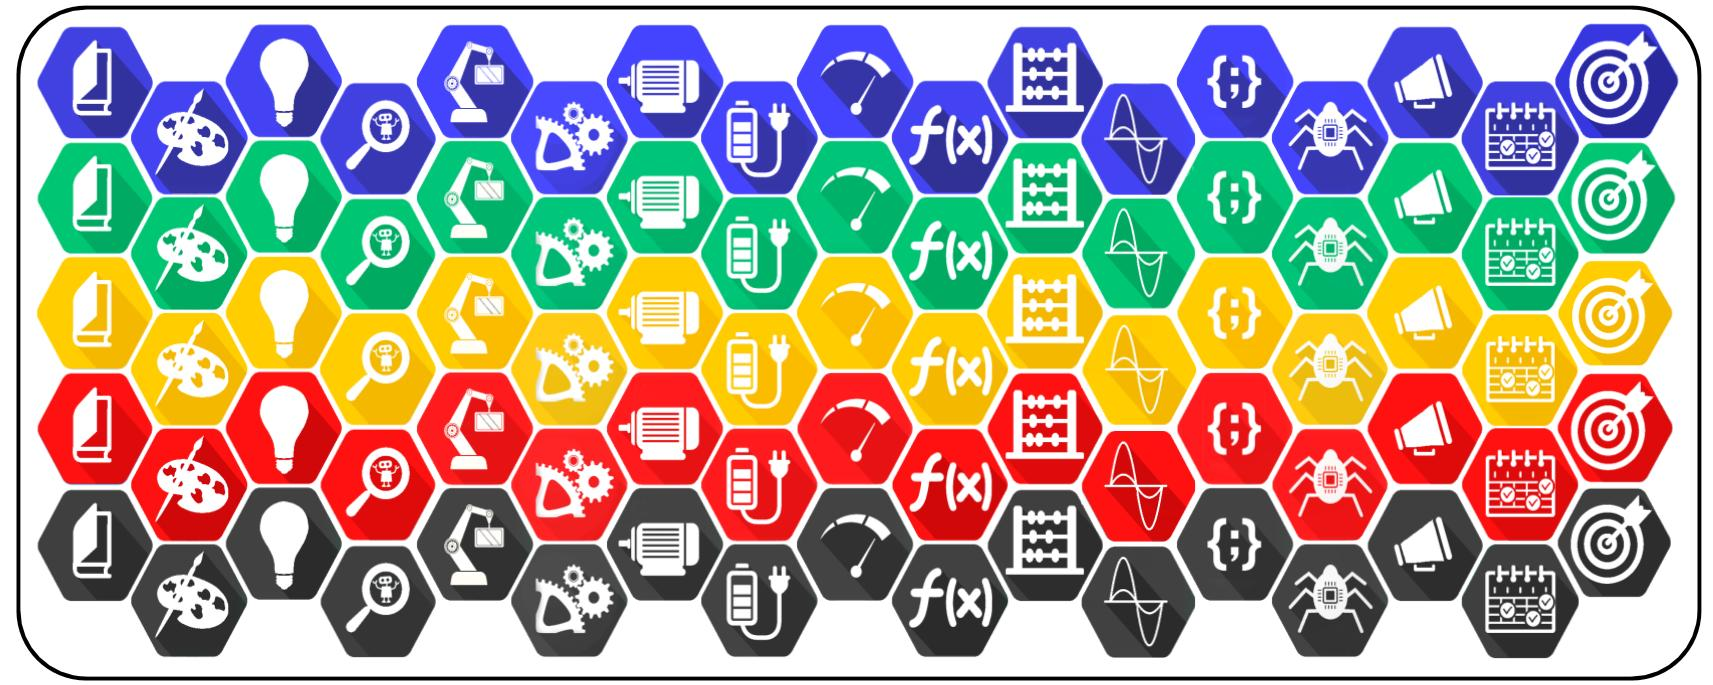
\includegraphics[width=\textwidth]{figuras/Icons/iconos.jpg}
   	\caption{Recopilación de los iconos diseñados y utilizados \completarCon{Añadir la diana}}
   	\label{fig:introduccion:iconos}
   	\immagesource{Autor}
\end{figure}